%\title{LaTeX Portrait Poster Template}
%%%%%%%%%%%%%%%%%%%%%%%%%%%%%%%%%%%%%%%%%
% a0poster Portrait Poster
% LaTeX Template
% for Humboldt-University Berlin 
% created by Patrick J�hnichen (patrick.jaehnichen@hu-berlin.de) on 29/6/2016
% licensed under CC BY-NC-SA 3.0 (http://creativecommons.org/licenses/by-nc-sa/3.0/)
%
% The a0poster class was created by:
% Gerlinde Kettl and Matthias Weiser (tex@kettl.de)
% 
% This template has been downloaded from:
% http://www.LaTeXTemplates.com
%
% License:
% CC BY-NC-SA 3.0 (http://creativecommons.org/licenses/by-nc-sa/3.0/)
%
%%%%%%%%%%%%%%%%%%%%%%%%%%%%%%%%%%%%%%%%%

%----------------------------------------------------------------------------------------
%	PACKAGES AND OTHER DOCUMENT CONFIGURATIONS
%----------------------------------------------------------------------------------------

\documentclass[a1,portrait]{a0poster}

\usepackage{multicol} % This is so we can have multiple columns of text side-by-side
\columnsep=.2\linewidth % This is the amount of white space between the columns in the poster
\columnseprule=2pt % This is the thickness of the black line between the columns in the poster

\usepackage[svgnames]{xcolor} % Specify colors by their 'svgnames', for a full list of all colors available see here: http://www.latextemplates.com/svgnames-colors

\usepackage{times} % Use the times font
%\usepackage[margin={5cm, 5cm, 1cm, 1cm}]{geometry}

%\usepackage{palatino} % Uncomment to use the Palatino font

\usepackage{graphicx} % Required for including images
\graphicspath{{figures/}} % Location of the graphics files
\usepackage{booktabs} % Top and bottom rules for table
\usepackage{amsfonts, amsmath, amsthm, amssymb} % For math fonts, symbols and environments
\usepackage{wrapfig} % Allows wrapping text around tables and figures

\usepackage{subfig}
%----------------------------------------------------------------------------------------
%	HU COLORS 
%----------------------------------------------------------------------------------------
\RequirePackage{hucolors}

\usepackage[font={footnotesize, color=hu_green, bf}, figurename=Fig., labelfont={bf}]{caption}% Required for specifying captions to tables and figures

\begin{document}

%----------------------------------------------------------------------------------------
%	POSTER HEADER 
%----------------------------------------------------------------------------------------

% The header is divided into two boxes:
% The first is 75% wide and houses the title, subtitle, names, university/organization and contact information
% The second is 25% wide and houses a logo for your university/organization or a photo of you
% The widths of these boxes can be easily edited to accommodate your content as you see fit
\setlength{\linewidth}{1450pt}

\begin{minipage}[t]{0.75\linewidth}
\huge \color{hu} \textbf{Bootstrapping the Support Vector Machine} \color{Black}\\[0.5cm] % Title
\large \textbf{Thomas Goerttler, Christian Koopmann, Patricia Craja}\\[0.5cm] % Author(s)
\large Department of Computer Science,\\
\large Machine Learning Group\\[0.4cm] % University/organization
\large Humboldt-University of Berlin, Germany\\
\normalsize \texttt{thomas.goerttler@gmail.com, c.k.e.koopmann@gmail.com, Patricia.craja@gmx.de}\\
\end{minipage}
%
\begin{minipage}[t]{0.24\linewidth}
\vspace{-50pt}
\raggedleft

\includegraphics[width=\linewidth]{husiegel_bw.pdf}%\hspace{\linewidth}
\vfill
\end{minipage}

\vspace{1cm} % A bit of extra whitespace between the header and poster content
\color{hu}
\noindent\makebox[\linewidth]{\rule{\paperwidth}{2pt}}
\color{Black}
%----------------------------------------------------------------------------------------
%\the\linewidth
\begin{multicols}{3} % This is how many columns your poster will be broken into, a portrait poster is generally split into 2 columns

%----------------------------------------------------------------------------------------
%	ABSTRACT
%----------------------------------------------------------------------------------------

\color{hu} % HU color for the abstract

\begin{abstract}
\footnotesize
The goal of this project is the analysis of the variance of Support Vector Machines (SVMs) and the relationship between this variance and other important aspects of the SVM. We provide a characterization of the variance of SVMs using the minimal distance of prediction points to the decision boundary and apply the bootstrap method in order to estimate the uncertainty of the prediction rule. The implementation of the Bootstrap (in Python) is done in a parallelized manner. Finally it will be shown how this variance is correlated with other characteristics of the SVMs, such as the regularization parameter and the number of support vectors, and with the balance of the training data set. This impact is analyzed for both Linear and Gaussian Kernel SVMs. Doing this for both simulated as well as real data sets produced very similar results. In this paper we therefore concentrate on showing the results obtained for simulated data. 
\end{abstract}
%----------------------------------------------------------------------------------------
%	INTRODUCTION
%----------------------------------------------------------------------------------------

\color{Black} 
\section*{Introduction}
\footnotesize
Support Vector Machines are one of the most successful methods of Machine Learning (\cite{steinwart_support_2008}). SVMs have many merits that distinguish them from other machine learning algorithms, including the speed of calculation, and the use of only two tuning parameters. Given a binary training data set, an SVM learning algorithm builds a model that predicts the unknown class for new input data, making it a non-probabilistic binary linear classifier (\cite{cristianini_introduction_2000}). SVM is based on a minimization problem, which seeks for a hyperplane in the feature space that optimally separates data points of two clusters.  By reducing non-linear complex decision problems to linear problems through application of the Kernel-Trick, they represent a computationally efficient way to tackle these problems. The dimension of the feature space is controlled by the choice of a specific Kernel function. Common Kernels are the Linear Kernel, the Gaussian Kernel (RBF) and the Polynomial Kernel.

SVMs based on certain Kernels (e.g. Gaussian RBF Kernel) are non parametric methods. Since the distribution of the underlying data is generally unknown, so is the finite sample distribution of these methods (\cite{hastie_elements_2005}).

There has been considerable research on the asymptotic distribution of SVMs, which have been shown to be asymptotically normally distributed under certain conditions. An alternative idea to estimate these distributions is to use Efrons empirical bootstrap (\cite{efron_introduction_1994}). The idea behind this method is to repeatedly draw samples with replacement from the full data according to the empirical distribution function of the data. Through the repeated calculation of the statistic of interest one can get an estimate of its distribution. For the SVM this estimate has been shown to be consistent under relatively mild conditions.
    
In the first section we will give an overview of the Problem to calculate the variance of the SVM. Then we will explain how we implemented the Bootstrap and the Data Simulation in order to estimate this variance. Once we estimated the variance we can finally analyze the influence of different parameters on this variance for both Linear and Gaussian Kernels.
%----------------------------------------------------------------------------------------
%	OBJECTIVES
%----------------------------------------------------------------------------------------

\color{Black} % Black color for the rest of the content

\section*{Problem}

In contrast to probabilistic classifiers which provide classification with a degree of certainty, SVMs only predict the most likely class that the sample should belong to.  

Since no adequate distribution theory exists, we apply the bootstrapping method to the SVM algorithm, i.e. drawing random training samples with replacement from the full training data set to train different SVMs. Through the repeated calculation of the predictions of the test data set we can estimate the prediction variance, which is an indicator of the degree of certainty of the SVM. 

Predictions however are only binary variables. Since they might be identical across all bootstrap samples, we use real valued substitutes such as the minimal distance of each prediction point to the decision boundary (Figure 1\label{fig1}) or the estimated probability of each prediction point to belong to the predicted class. After testing both substitutes we decided to use the minimal distance to the decision boundary as it is easier to understand how these values are calculated. 

\begin{center}\vspace{1cm}
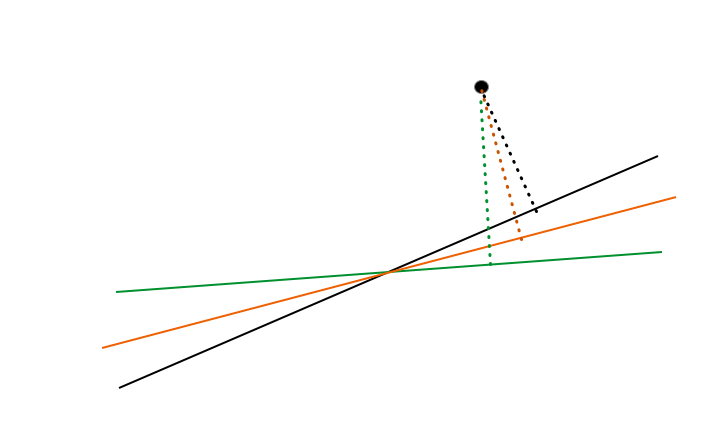
\includegraphics[width=0.8\linewidth]{abb/distances.jpg}
\captionof{figure}{The minimal distance of a prediction point to each hyperplance is considered.}
\end{center}\vspace{1cm}

%----------------------------------------------------------------------------------------
%	MATERIALS AND METHODS
%----------------------------------------------------------------------------------------

\section*{Implementation}



\subsection*{Bootstrapping}
In order to calculate the variance of the predictions we use bootstrap samples. We start by training the SVM on the full training data and will call this SVM the \textit{Full SVM}. Then we draw $N$ random bootstrap samples with replacement (\cite{christmann_bootstrap_2013}) from the full training data and train the SVM $N$ times on each bootstrap sample in a parallelized manner. That way we get $N$ different SVMs that predict for each input of the test data of size $n$ to which class it belongs. Figure 2 \label{fig2} illustrates the different results obtained for the linear Kernel for perfectly separated data (a and c) and not perfectly separated data (b and d), as well as for a smaller size of the training data (a and b) and a bigger one (c and d). We observe that the variance is smaller if the data is perfectly separated and if the training data contains more observations.

The $n$ distances of each point in the test data set from the decision boundary can be seen as random variables. For the $N$ SVMs we obtain $N$ different values of these random variables and can calculate their variance. We take the average of these $n$ variances as an indicator for the variance of the \textit{Full SVM}. Therefore our Bootstrap Method uses as input the training data set, the test data set, SVM-Parameters, and the number $N$ of bootstrap replications and it returns the \textit{Full SVM}, its number of support vectors as well as its variance.

\begin{center}\vspace{1cm}
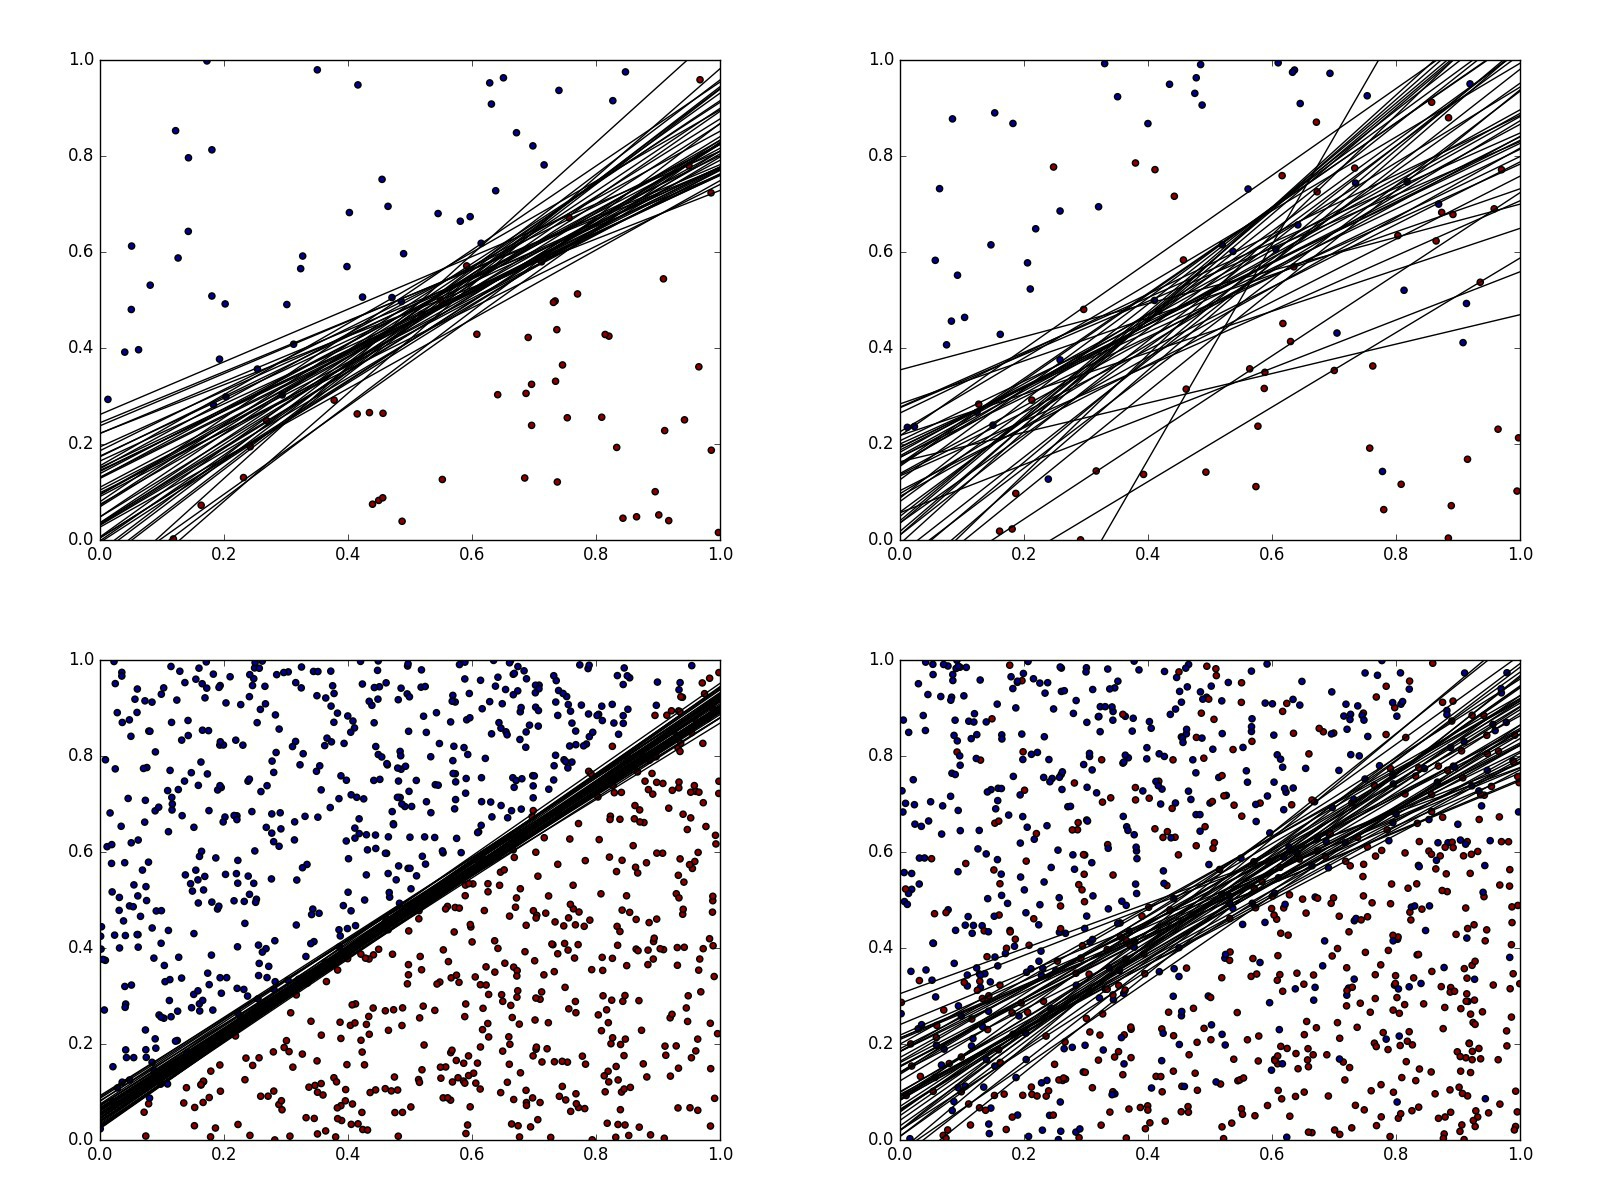
\includegraphics[width=1\linewidth]{abb/pic.jpg}
\captionof{figure}{In each picture 100 hyperplances are plotted based on samples. In (a) and (c) the data are perfectly separated whereas in (b) and (d) small errors occur. In (a) and (b) we used 100 observations in the training data and in (c) and (d) we used 1000.}
\label{fig3}
\end{center}\vspace{1cm}


\paragraph{Parallelization:} In order to make the bootstrapping efficient, it is parallelized. A pool of processes is created to carry out tasks submitted to it using the Python \texttt{Pool} class. Each process trains a certain numbers of SVMs on bootstrap samples and calculates the distances for each test point. The results from each process are then collected in an array which is used to calculate the statistics mentioned above. Since the training of each SVM is independent of the others, the parallelization of this algorithm is relatively straight forward.


\subsection*{Data Simulation}
For the Data Simulation we use two different approaches, the Hyperplane- and the Centroid- Approach. For both we randomly draw $n$ observations for each of the input variables $x$ from a normal distribution. The Hyperplane-Approach calculates the labels using the formula $y= sign(c+ w^T x + error)$, given the Hyperplane-Parameter $w$, a constant $c$ as well as the error distribution, whereas the Centroid-Approach calculates the labels using the formula $y= sign(c + a_1*(d(x,z_1)^{-1}... + error)$ given the Centroid- Locations $z_i$, the Centroid- Parameters  $a_i$, a constant $c$ and a distance function $d(a,b)$.
To change the number of support vectors of a data set the variance of the error is modified, whereas the intercept controls the balance of the data set.

%	RESULTS 
%----------------------------------------------------------------------------------------

\section*{Results}


In this section we will show how the prediction variance is correlated with other aspects of the SVM, such as the regularization parameter $C$, the balance of the training data set and the number of support vectors of the original \textit{Full SVM}. Analyzing this impact for both Linear  and Gaussian Kernel SVMs produced the following results:

\begin{center}\vspace{1cm}
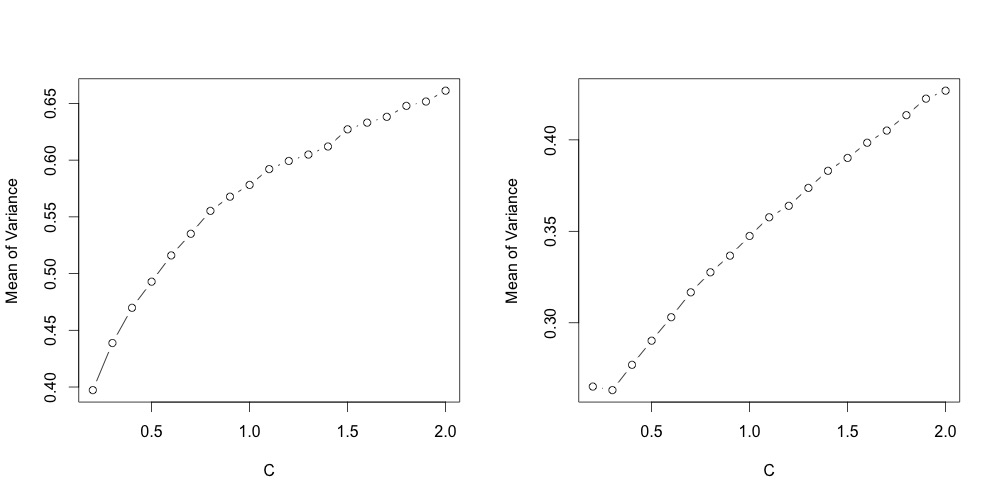
\includegraphics[width=1\linewidth]{abb/c.jpg}
\captionof{figure}{Relation between the variance mean and the regularization parameter $C$. The y-axis represents the mean of the variance of 20 different data sets for each value of $C$. The size of each data set is n=100 and N=1000 replications are done. (a) corresponds to the Linear, (b) to the Gaussian Kernel.}
\label{fig3}
\end{center}\vspace{1cm}



\subsection*{Influence of the regularization parameter C}
\paragraph{Observations:}
As seen in Figure 3\label{fig3}, by changing the regularization parameter $C$ we obtained similar results for both Linear and Gaussian Kernel SVMs. The higher the regularization parameter $C$, the higher will be the variance of the SVM-predictions. The parameter $C$ is therefore positively correlated with the variance.
\paragraph{Interpretation:}
The parameter C controls the trade off between errors of the SVM on training data and margin maximization. To avoid overfitting, the SVM employs regularization and controls the amount of regularization by the constant $C$ (\cite{hastie_elements_2005}). A high value of $C$ corresponds to low regularization, i.e. lower size of slack variables and therefore higher overfitting, which means that the SVM fits the training data too well but does not generalize to new data and therefore the variance of the predictions of our test data rises.

Figure 3 shows this relation for values between 0 and 2 of the parameter $C$ 
for Linear and Gaussian Kernels. Because each value of $C$ corresponds to a different \textit{Full SVM}, we calculated the average of 20 SVM variances for each value of C, i.e. 20 test data set variances as explained at the beginning (using $N$=1000 Bootstrap Replications, and $n$=100 data points).

\begin{center}\vspace{1cm}
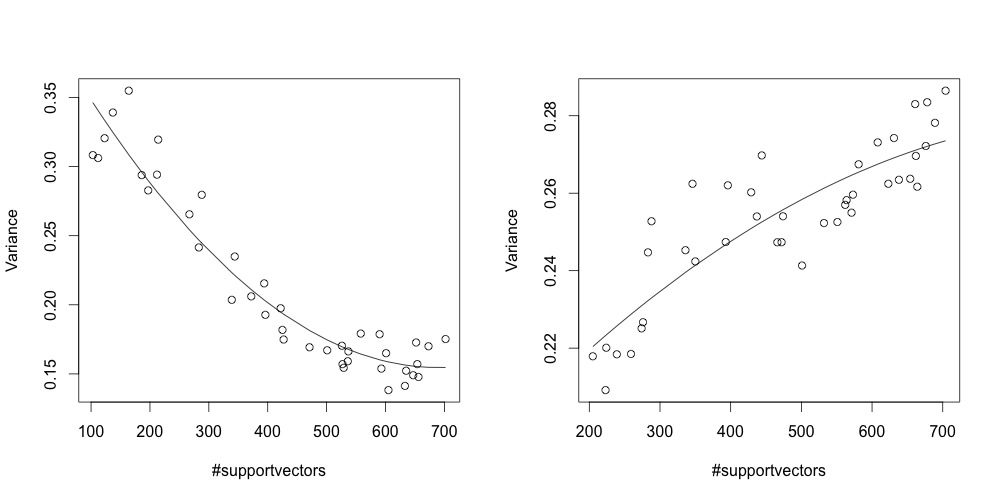
\includegraphics[width=1\linewidth]{abb/n_support.jpg}
\captionof{figure}{Relation between the variance and the number of support vectors. The data set size is n=1000 and N=500 replications are done. (a) corresponds to the Linear, (b) to the Gaussian Kernel.}
\label{fig4}
\end{center}\vspace{1cm}


\subsection*{Influence of the number of support vectors}
\paragraph{Observations:}
In Figure 4\label{fig4} it can be seen, that changing the number of support vectors for the \textit{Full SVM} we obtained different results for Linear and Gaussian Kernels. For the Linear Kernel, the variance of the SVM decreases with an increase in support vectors, whereas for the Gaussian Kernel the variance increases with more support vectors. The number of support vectors is therefore negatively correlated with the variance of the Linear Kernel and positively correlated with the variance of the Gaussian Kernel.
\paragraph{Interpretation:}
The number of support vectors controls the slack variables of the soft margin SVM. A high number of support vectors implies larger margins and higher slack variables. Training the Linear SVM on the bootstrap samples is therefore more robust and the variance of the decision boundary as well as the distance from each point of the test data set to the decision boundary has smaller variation.
For Gaussian Kernels, a higher number of support vectors might imply overfitting on the training data set and therefore bad generalization to new data which could be the reason why the variance of the predictions of our test data rises.

\begin{center}\vspace{1cm}
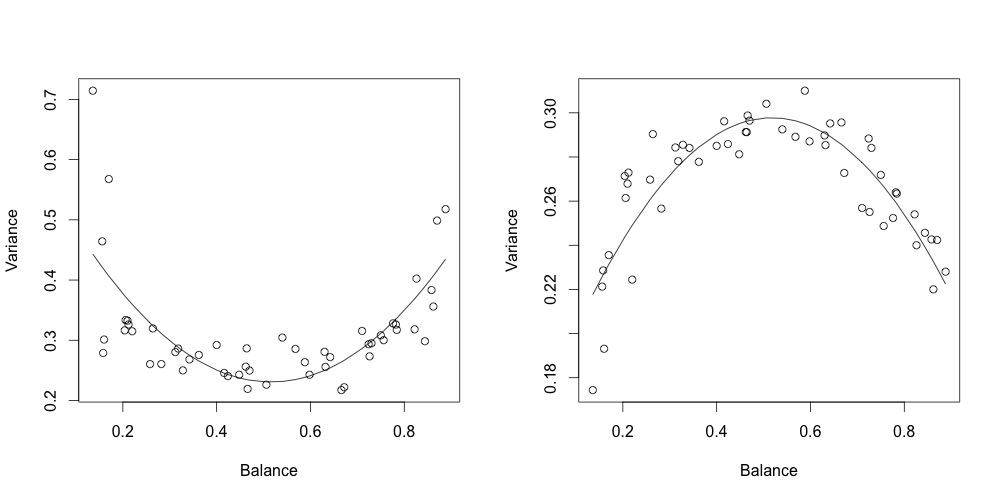
\includegraphics[width=1\linewidth]{abb/balance.jpg}

\captionof{figure}{Relation between variance and balance of the data. The data set size is n=500 and N=1000 replications are done. (a) corresponds to the Linear, (b) to the Gaussian Kernel.}
\label{fig5}
\end{center}\vspace{1cm}



\subsection*{Influence of the balance of the training data set}

\paragraph{Observations:}
Changing the balance of the training data set, from which the samples are taken, we obtain different results for the Linear and Gaussian Kernels, as  seen in Figure 5\label{fig5}. As expected the resulting graph is symmetric around 0.5 for both kernels. For the Linear Kernel, the variance of the SVM rises when the data is unbalanced and it is minimal for perfectly balanced data. However, for the Gaussian Kernel the maximal variance is attained for perfectly balanced data, and it drops for unbalanced data. 
\paragraph{Interpretation:}
In the linear case the variance is especially high, when one class is very small compared to the other class. The location of the linear hyperplane is on the few points from the smaller class. Depending on  which points are sampled from this class, the decision boundary and therefore the distance of test points to this boundary might vary dramatically.
The Gaussian Kernel shows exactly the opposite results. This occurs because the Gaussian Kernel tends to overfit the data on the training data sets (\cite{hastie_elements_2005}). We have taken 1000 samples from the data set. If the data is perfectly balanced, more different samples of the smaller group are possible. Therefore the hyperplanes differ more. If the smaller class is very small, the sample from the smaller class can not differ that much from each other.
Nevertheless it can be obtained, that the effect is extremely high in the tails and rather small between a balance of 0.3 to 0.7 .



%----------------------------------------------------------------------------------------
%	CONCLUSIONS
%----------------------------------------------------------------------------------------

\color{hu_red} % HU red color for the conclusions to make them stand out

\section*{Conclusions}

\begin{itemize}
\item Calculating the variances by using bootstrap samples seems to be a quite good idea to calculate a variance. 
\item The variance of distances of test points seems to be a good indicator for the robustness of the SVM as shown in Figure 2 \label{fig2}.
\item The results of changing the $C$-parameter are not surprising but confirm the strength of the variance estimator.
\item Especially interesting and to some degree counterintuitive are the different effects of support vectors and data balance on the Kernels.
\item Overall the bootstrapping method has once again shown its value for situations where classical methods of statistical inference are not available.
\end{itemize}

\color{Black} % Set the color back to Black for the rest of the content

%----------------------------------------------------------------------------------------
%	FORTHCOMING RESEARCH
%----------------------------------------------------------------------------------------

\section*{Forthcoming Research}

Further interesting analysis would be to look for the influence of the dimensionality on variances. The influence of other tuning parameters such as the gamma parameter of the RBF-Kernel or the degree of Polynomial Kernels could be interesting areas of inquiry. Also in this context we could only give rough explanations for the findings. More accurate explanations might be found when analysing one of the aspects in more detail. Also despite the parallelization of the algorithm the procedures are still computationally very intensive. Using more sample computing resources (and thereby increasing both the number of observations as well as bootstrap samples) would probably lead to even more reliable results.

 %----------------------------------------------------------------------------------------
%	REFERENCES
%----------------------------------------------------------------------------------------

\nocite{*} % Print all references regardless of whether they were cited in the poster or not
\bibliographystyle{plain} % Plain referencing style
\bibliography{sample} % Use the example bibliography file sample.bib

%----------------------------------------------------------------------------------------
%	ACKNOWLEDGEMENTS
%----------------------------------------------------------------------------------------

%\section*{Acknowledgements}

%Etiam fermentum, arcu ut gravida fringilla, dolor arcu laoreet justo, ut imperdiet urna arcu a arcu. Donec nec ante a dui tempus consectetur. Cras nisi turpis, dapibus sit amet mattis sed, laoreet.

%----------------------------------------------------------------------------------------

\end{multicols}
\end{document}